\documentclass[a4paper,12pt]{article}

\usepackage{cmap}          % поиск в PDF
\usepackage{mathtext}         % русские буквы в формулах
\usepackage[T2A]{fontenc}      % кодировка
\usepackage[utf8]{inputenc}      % кодировка исходного текста
\usepackage[english,russian]{babel}  % локализация и переносы
\usepackage[left=2cm,right=2cm,top=2cm,bottom=2cm]{geometry}
\usepackage{amsfonts,amssymb,amsthm,mathtools} % AMS
\usepackage{amsmath}
\usepackage{icomma} % "Умная" запятая: $0,2$ --- число, $0, 2$
\usepackage{graphicx}
\usepackage{wrapfig} % картинка в тектсе
\usepackage{caption} % убирается номер у подписей caption*{}
\usepackage{csquotes} % цитаты
\usepackage{multirow} % для жестких таблиц
\usepackage{hhline}
\usepackage{indentfirst} % абзацный отступ после section
\usepackage{epigraph} % эпиграф
\usepackage{tikz}
\usepackage{pgfplots}
\usepackage[export]{adjustbox}
\usepackage{tabularx}
\usepackage{float}
\usepackage{longtable}



\title{\textbf{Определение моментов инерции твердых тел с помощью трифилярного подвеса. (1.2.3)}}
\author{Зайнуллин Амир}


\begin{document}
\maketitle

\section{Аннотация}
    \textbf{Цели работы:} измерение момента инерции тел и сравнение результатов с расчетми по теоретиеским формулам; проверка аддитивноски моментов инерции и справедливости формулы Гюйгенса-Штейнера. \par
	\textbf{Оборудование:} трифилярный подвес, секундомер, счетчик числа колебаний, набор тел, момент инерции которых надлежит измерить. \par

\section{Теоретические сведения}
    \textbf{Упрощения:} При колебаниях не учитываются потери энергии на трение о воздух. \\
    Закон сохранения энергии, учитывая наше упрощение, имеет вид:

    
    $$\frac{I\dot \varphi^2}{2} + mg(z_0-z) = E$$
    

    Здесь $I$ -- момент инерции платформы вместе с исследуемым телом, $m$ -- масса платформы с телом, $\varphi$ -- угол поворота платформы от положения равновесия системы, $z_0$ -- координата по вертикали центра нижней платформы $O'$  при равновесии ($\varphi = 0$), $z$ -- координата той же точки при некотором угле поворота $\varphi$. \par
    Воспользуемся системой координат $x, y, z$, связанной с верхней платформой, как показано на Рис. 1. Координаты верхнего конца одной из нитей подвеса точки $C$ в этой системе -- $(r, 0, 0)$. Нижний конец данной нити $C'$, находящийся на нижней платформе, при равновесии имеет координаты $(R, 0, z_0)$, а при повороте платформы на угол $\varphi$ эта точка переходит в $C''$ с координатами $(Rcos\varphi, Rsin\varphi, z)$. расстояние между точками $C$ и $C''$ равно длине нити, поэтому, после некоторых преобразований, получаем:
    
    $$(R\cos\varphi - r)^2 + R^2\sin^2\varphi + z^2 = L^2$$
    $$ z^2 = L^2 - R^2 - r^2 + 2Rr\cos\varphi \approx z^2_{0} - 2Rr(1 - \cos\varphi) \approx z^2_{0} - Rr\varphi^2 $$
	$$ z = \sqrt{z^2_{0} - Rr\varphi^2} \approx z_{0} - \frac{Rr\varphi^2}{2z_{0}} $$ \par
    Подставляя $z$ в закон сохранения энергии, получим:
    $$\frac{1}{2}I\dot\varphi^2 + \frac{mgRr}{2z_0}\varphi^2 = 0$$ \par
    Дифференцируя по времени, получаем уравнение колебаний:
    $$I\ddot\varphi^2 + \frac{mgRr}{z_0}\varphi^2 = 0$$
    $$\varphi = \varphi_0 sin \left(\sqrt{\frac{mgRr}{Iz_0}}t + \theta\right)$$ \par
    Здесь амплитуда $\varphi_0$ и фаза $\theta$ колебаний определяются начальными условиями. Период кртуильных полебаний нашей системы равен:
	$$T = 2\pi \sqrt{\frac{Iz_0}{mgRr}}$$ \par
    Из формулы для периода получаем:
    $$I = \frac{mgRrT^2}{4 \pi^2z_0} = kmT^2$$ \par
	где $k = \frac{gRr}{4\pi^2z_0}$ -- величина, постоянная для данной установки.

\section{Методика измерений}
    \begin{wrapfigure}{l}{7cm}
        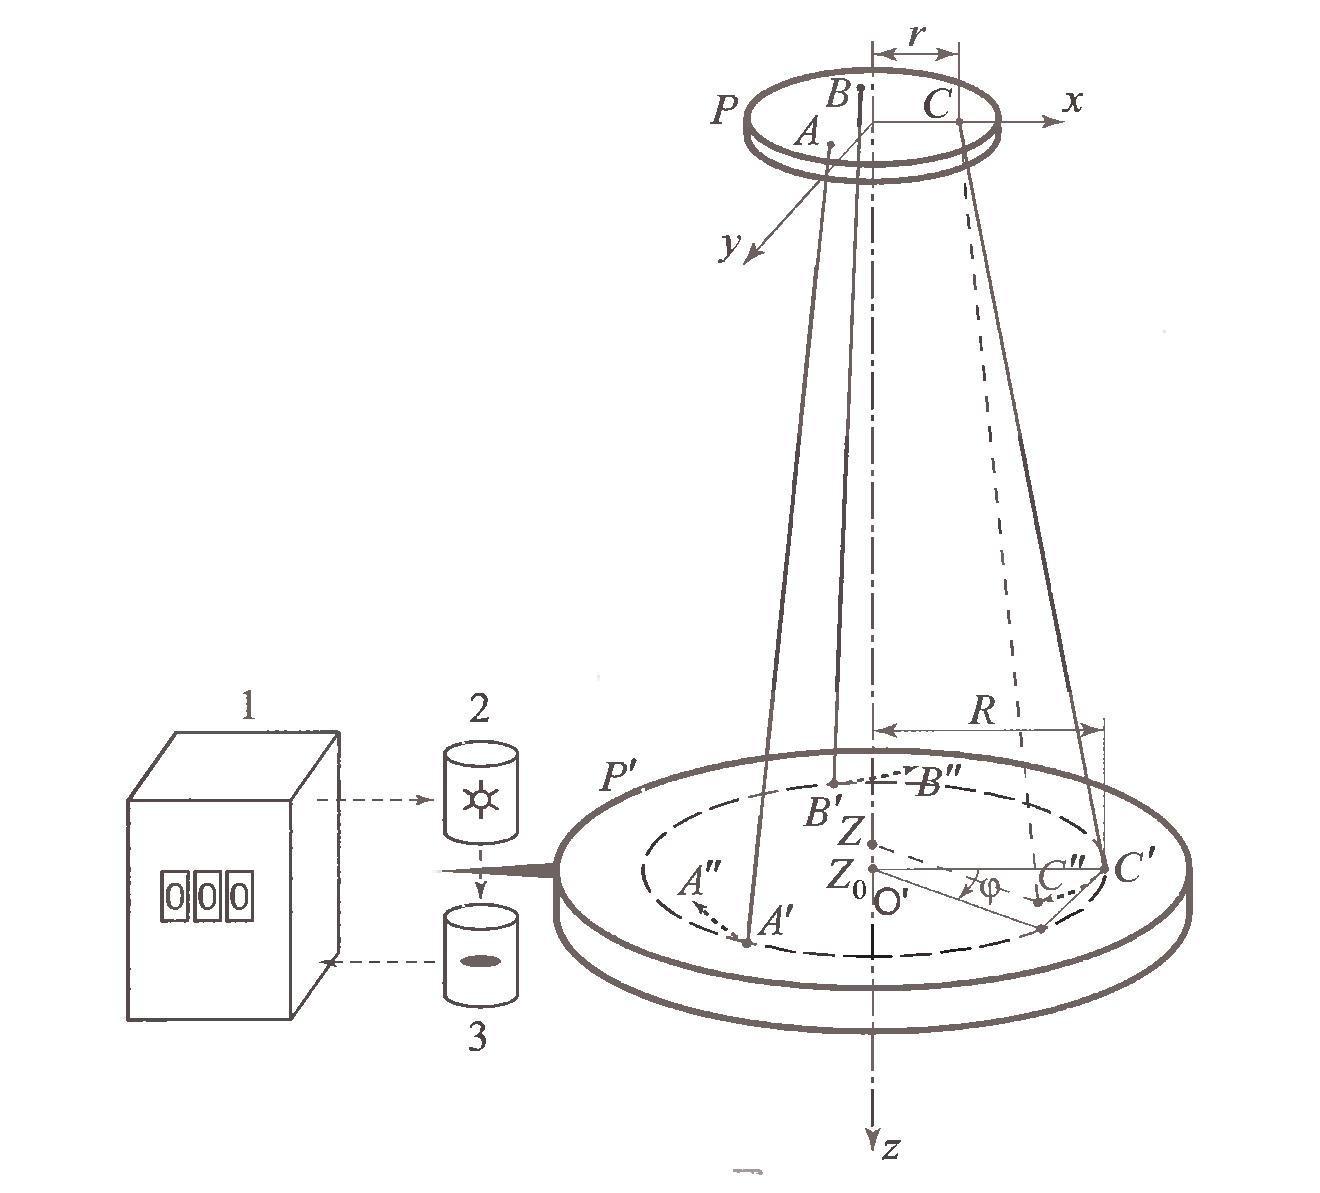
\includegraphics[width=1\linewidth]{1.2.3 ustan.png}
        \caption{Трифилярный подвес}
    \end{wrapfigure}

    Для наших целей будем использовать трифилярный подвес. Он состоит из укрепленной на некоторой высоте неподвижной платформы $P$ и подвешенной к ней на трех симметрично расположеных нитях $AA'$, $BB'$ и $CC'$, вращающейся платформы $P'$. \par
    Чтобы не вызывать дополнительных раскачиваний, лучше поворачивать верхнюю платформу, укрепленную на неподвижной оси. После поворота верхняя платформа остается неподвижной в течение всего процесса колебний. После того, как нижняя платформа $P'$ оказывается повернутой на угол $\varphi$ относительно верхней платформы $P$, возникает момент сил, стремящийся вернуть нижнюю платформу в положение равновесия, при котором относительный поворот платформ отсутствует. В результате платформа совершает крутильные колебания. 


\section{Используемое оборудование}
    Секундомер измеряет время с абсолютной погрешностью $\sigma_T^{\text{сист}} = 0,001$ с.
    \subsection*{Параметры установки и коэффицент $k$}
    Работа выполнялась на установке №8, ее параметры указаны в таблице 1.
    \begin{table}[H]
	    \begin{center}
		    \begin{tabular}{|c|c|c|c|c|}
			    \hline
			    $m \text{, г}$  & $R\text{, мм}$ & $r\text{, мм}$ & $L\text{, см}$ & $z_0\text{, см}$\\
			    \hline
			    1004,8 & 114,1 & 30,5 & 217,6 & 217,1\\
			    \hline
			    \hline
			    $\sigma_m \text{, г}$  & $\sigma_R\text{, мм}$ & $\sigma_r\text{, мм}$ & $\sigma_L\text{, см}$ & $\sigma_{z_0}\text{, см}$\\
			    \hline
			    0,5 & 0,5 & 0,3 & 0,1 & 0,1\\
			    \hline 
		    \end{tabular}
	    \caption{Параметры установки}
        \end{center}
	\end{table}
    По полученным данным вычислим постоянную для конструкции №3:
	$$k = \frac{gRr}{4\pi^2z_0} \approx 3,98\cdot 10^{-4} \frac{м^2}{с^2}$$
    Погрешность $k$ будет равна:
	$$\sigma_k = k \cdot \sqrt{\left( \frac{\sigma_R}{R}\right)^2 + \left( \frac{\sigma_r}{r}\right)^2 + \left( \frac{\sigma_{z_0}}{z_0}\right)^2} \approx 0,04 \cdot 10^{-4} \frac{\text{м}^2}{\text{с}^2}$$
	
\section{Результаты измерений и обработка данных}
    \subsection*{Момент инерции ненагруженной платформы}
    Сначала определим период колебаний ненагруженной платформы.
    \begin{table}[H]
        \begin{center}
            \begin{tabular}{|c|c|c|}
                \hline 
                $№$ & Время колебаний $T_n, с$ & Период колебаний $T, с$\\
                \hline
                1 & 44,705 & 4,4705\\
                \hline 
                2 & 44,685 & 4,4685\\
                \hline 
                3 & 44,63 & 4,463\\
                \hline
            \end{tabular}
        \end{center}
    \end{table} 
    Тогда средний период колебаний $T_\text{ср} = 4,467$ с. Определим погрешность.
    $$\sigma_T^{\text{случ}} =\frac{1}{N}\sqrt{\sum_{i=1}^{N}\left( T_\text{ср} - T_i \right)^2 } \approx 0,003 \text{ с}$$ 
    $$\sigma_T = \sqrt{\sigma_\text{случ}^{2} + \sigma_{\text{сист}}^{2}} \approx 0,003\text{ с}$$
    Найдем момент инерции ненагруженной платформы
    $$I_\text{пл} = kmT_\text{ср}^2 = 7,98 \cdot 10^{-3} \text{ кг} \cdot \text{м}^2$$
    $$\varepsilon = \sqrt{ \left(\frac{\sigma_k}{k}\right)^2 +\left(\frac{\sigma_m}{m}\right)^2 + \left(2\frac{\sigma_T}{T}\right)^2} = 0,01$$
    $$\sigma_\text{I\text{пл}} = I_\text{пл} \varepsilon = 0,08 \cdot 10^{-3} \text{ кг} \cdot \text{м}^2$$
    Значит, с данной установкой мы можем мы можем определять момент инерции тел с точностью 1\% и $I_\text{пл} = \left(7,98 \pm 0,08\right) \cdot 10^{-3} \text{ кг} \cdot \text{м}^2$
    
\subsection*{Определение моментов инерции различных тел. Аддитивность моментов инерции}
    Измерим периоды колебаний платформы с различными телами таким же образом, как и для ненагруженной платформы, а именно -- 3 измерения по 10 колебаний для каждого набора тел, получаем:
	\begin{table}[H]
        \begin{center}
            \begin{tabular}{|c|c|c|c|c|c|c|c|c|}
                \hline 
                Набор тел & $t_1, с$ & $t_2, с$ & $t_3, с$ & $t_\text{ср}, с$ & $T, с$ & $m_0$, г & $I \cdot 10^{-3}$,$\text{ кг} \cdot \text{м}^2$ & $\sigma_I \cdot 10^{-3}\text{, кг} \cdot \text{м}^2$\\
                \hline
                Пл.+Крыш. & 36,702 & 36,671 & 36,594 &  36,656  & 3,6656 & 2127,7 & 11,378 & 0,114\\
                \hline 
                Пл.+Труба & 43,04 & 42,95 & 42,89 & 42,96 & 4,296 & 1986,5 & 14,592 & 0,146\\
                \hline 
                Оба тела & 38,279 & 38,136 & 38,192 & 38,202 & 3,8202 & 3109,4 & 18,061 & 0,180\\
                \hline 
            \end{tabular}
            \caption{Моменты инерции платформы с различными телами}
        \end{center}
    \end{table} 

    Для подтверждения аддитивности необходимо показать,что выполняются условия:
    $$I_\text{пл+кр} = I_\text{пл} + I_\text{кр}$$
    $$I_\text{пл+тр} = I_\text{пл} + I_\text{тр}$$
    $$I_\text{пл+кр+тр} = I_\text{пл} + I_\text{кр} + I_\text{тр}$$

    Из таблицы и формул мы можем найти момент инерции цилиндра и кольца, учитывая что погрешности момента инерции диска и вычисленных далее будут складываться: $I_\text{кр} = I_\text{пл+кр} - I_\text{пл} = \left(3,398 \pm 0,194\right) \cdot 10^{-3} \text{ кг $\cdot$ $\text{м}^2$ }$, а $I_\text{тр} = I_\text{пл+тр} - I_\text{тр} = \left(6,612 \pm 0,226\right) \cdot 10^{-3} \text{ кг $\cdot$ $\text{м}^2$}$.
    Тогда, для доказательства аддитивности, проверим последнее уравнение. Оно выполняется, следовательно моменты инерции аддитивны.
    
    Теперь сравним полученные нами моменты инерциии для тел, и их теоретические значения. Для крышки: $I_\text{кр} = \frac{1}{2}m_\text{кр}R_\text{кр}^2$. $R_\text{ц} = 10,96\text{, см}$, тогда $I_\text{ц} = 2,135 \text{,  кг $\cdot$ $\text{м}^2$ $\cdot 10^{-3}$}$, что подтверждает экспериментальное значение.
	Для кольца же: $I_\text{к} = m_\text{к}R_\text{к}^2$. Так как данное кольцо не идеально тонко, то $R_\text{к} = \frac{D_\text{внут} + h}{2}$, где $h = 0,41 \text{, см}$, а $D_\text{внут} = 15,08\text{, см}$, тогда $R_\text{к} = 7,745 \text{, см}$. Получаем, что $I_\text{к} = 4,487\text{,  кг $\cdot$ $\text{м}^2$ $\cdot 10^{-3}$}$, что тоже совпадает с полученным экспериментально значением.
\end{document}
